\section{Concepts and Related Work}
\label{sec:background}

\subsection{Agglomerative Clustering}
\label{subsec:agglomeration}

This is a method of grouping observations or data points in which
the most similar are grouped together right away, then the slightly less
similar are added to those clusters. As clusters grow they can also glom on
to each other. This process of similar observations and clusters
repeatly combining to form larger clusters is
\textbf{\href{
https://en.wikipedia.org/w/index.php?title=Hierarchical_clustering&section=3
}{agglomerative clustering}}.
It's also called hierarchical clustering because when you trace the lineage
observations and mini-clusters combining, it forms a tree showing
the hierarchy of similarity between them. 

\subsection{Multi-membership Clustering}
\label{subsec:multimembership}

Ziptie is an unusual variant of agglomerative clustering where an item
can belong to multiple clusters. Here the ziptie analogy of
Figure~\ref{fig:multimember} can be helpful.
In a set of wires, imagine pulling out five of them and wrapping them
with one ziptie. Then imagine taking just two of those five, selecting another
two loose wires, and wrapping those four with another ziptie.
Two of the wires are included in both zipties. Those represent elements
with multiple cluster membership.

\begin{figure}[ht]
\vskip 0.0in
\begin{center}
\centerline{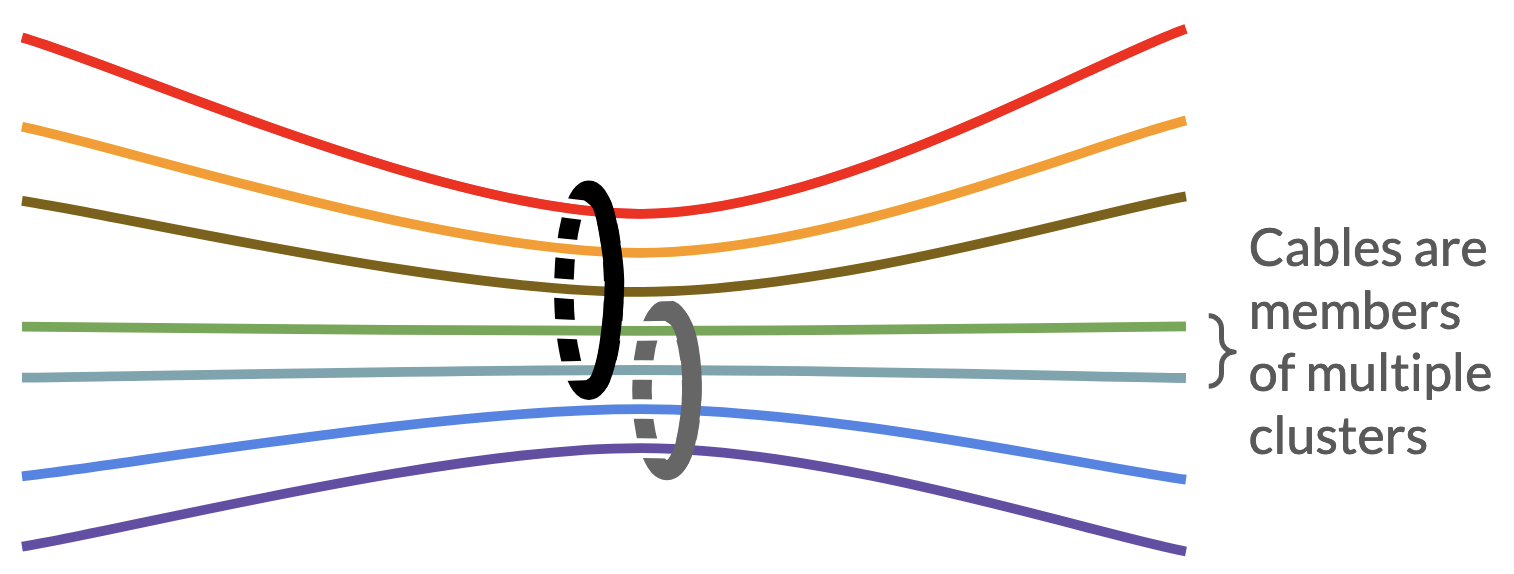
\includegraphics[width=3.0in]{images/multimember.png}}
\caption{Clustering with multiple membership.}
\label{fig:multimember}
\end{center}
\vskip -0.2in
\end{figure}

\subsection{Feature Learning}
\label{subsec:featurelearning}

Feature engineering is the practice of cleverly combining several features
to get at information that none of them could provide on their own.
For example, the $x$- and $y$-velocities of an object can be combined
to give its overall speed, or specific
patterns in a $3 \times 3$ collection of
pixels can be used to detect edges.
Feature learning, also known as \textbf{
\href{https://en.wikipedia.org/w/index.php?title=Feature_engineering&section=3}
{automated feature engineering}}, is when features are generated through
heuristics or the result of algorithms.
There are a collection of
\textbf{
\href{https://en.wikipedia.org/w/index.php?title=Feature_engineering&section=5}
{open source tools}} for this, which largely
focus on time series data sets.

Feature learning is also referred to as \textbf{
\href{https://en.wikipedia.org/wiki/Feature_learning}{representation learning}}.
\textbf{\href
{https://en.wikipedia.org/w/index.php?title=Feature_learning&section=6}
{Principal components analysis}} (PCA) is the poster child for unsupervised
representation learning. PCA resembles Ziptie in that it finds combinations
of features that tend to co-occur. PCA is focused on \textit{dimensionality
reduction} in that its goal is to reduce the total number of features used
to a small set that distills out most of the informtion in the data.

\subsection{Feature Agglomeration}
\label{subsec:featureagg}

On its surface,
scikit-learn's
\href{https://scikit-learn.org/stable/auto_examples/cluster/plot_digits_agglomeration.html#sphx-glr-auto-examples-cluster-plot-digits-agglomeration-py}
{feature agglomeration}
\footnote{Pedregosa, F., Varoquaux, G., Gramfort, A., Michel, V.,
Thirion, B., Grisel, O., Blondel, M., Prettenhofer, P.,
Weiss, R., Dubourg, V., Vanderplas, J., Passos, A.,
Cournapeau, D., Brucher, M., Perrot, M., Duchesnay, E. (2011)
Scikit-learn: Machine Learning in Python. Feature agglomeration.
\textit{JMLR}, 12, 2825–2830.}
is similar to Ziptie.
It uses agglomerative clustering to group
features into larger groups of features. However, it is different in
some important ways, which are illustrated in
Section~\ref{subsec:whycoactivation}.

\subsection{Sparse Coding}
\label{subsec:sparsecoding}

Ziptie is actually an example of
\textbf{\href{https://en.wikipedia.org/wiki/Sparse_dictionary_learning}
{sparse coding}} or \textit{sparse dictionary learning}, a family of methods
for learning concise ways to represent data. 

The goal of sparse coding is to represent using as few features as possible.
To do this, sparse coding methods often learn an
\textit{overcomplete dictionary of basis functions}.
Basis functions are combinations of features, the elements of a
dictionary that the sparse coding method uses to re-express each
observation.
Overcomplete means that the method learns several ways to express
the same observation. This allows it the sparsest one, the one with
the fewest non-zero elements.

A culinary example of sparse coding is "Moose Tracks" flavor ice cream.
It could just as accurately be described as "vanilla with small
peanut butter cups and fudge ripples". The name "Moose Tracks" is
superfluous; it means exactly the same thing.
Its existence shows overcompleteness in the dictionary
of ice cream flavor names. But it allows for concise representation,
a sparse coding of the 

\begin{figure}[ht]
\vskip 0.2in
\begin{center}
\centerline{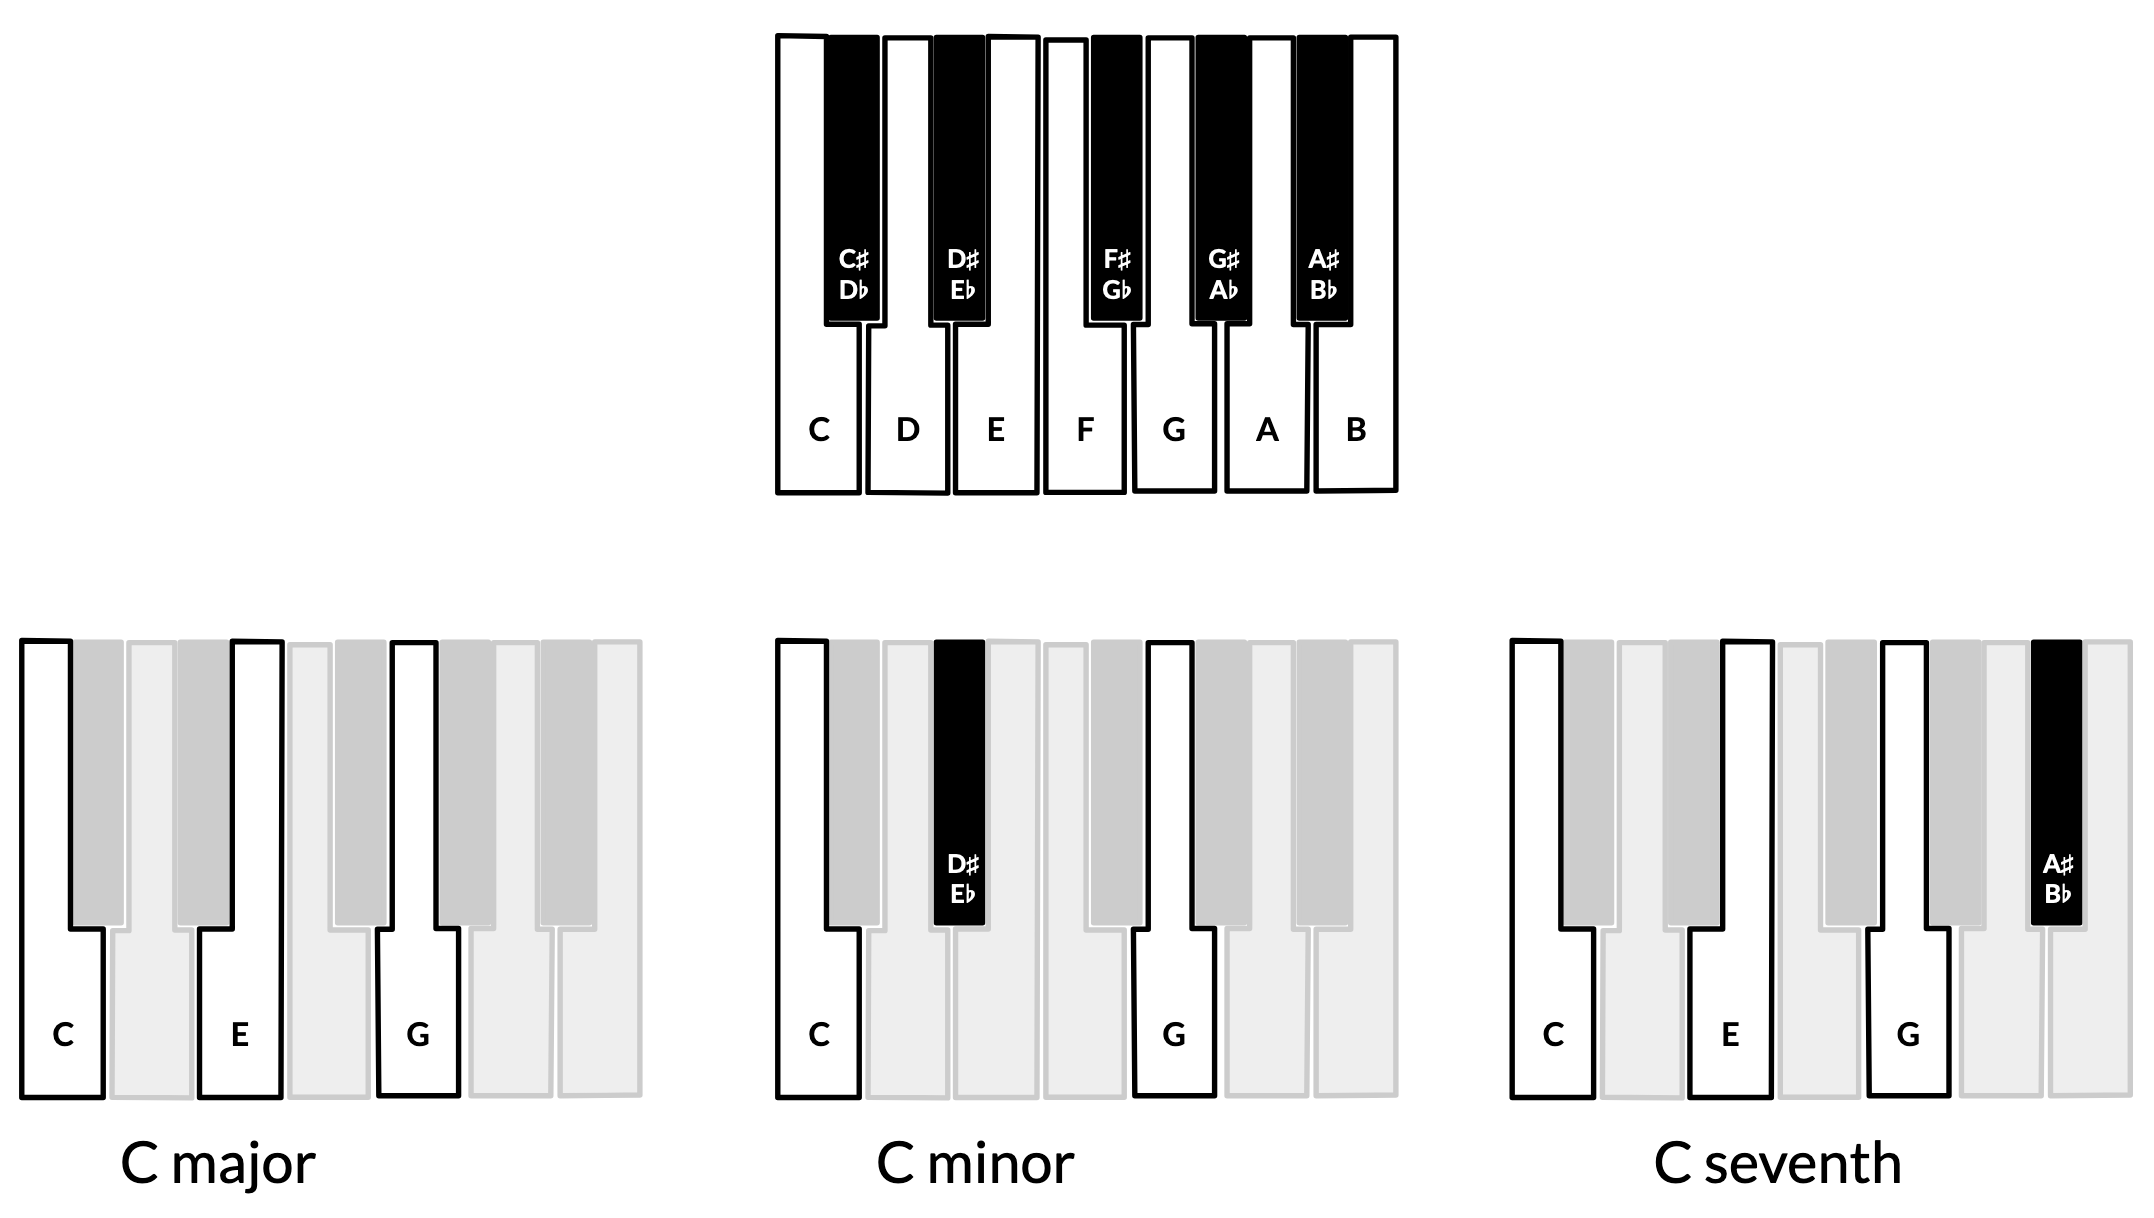
\includegraphics[width=3.25in]{images/chords.png}}
\caption{Piano chords as a sparse coding}
\label{fig:chords}
\end{center}
\vskip -0.2in
\end{figure}

\subsection{$\ell^0$ vs $\ell^1$ Norms}
\label{subsec:sparsenorms}

L0 sparse coding

Computer vision, anomaly detection
https://arxiv.org/abs/2104.04289

L0-KSVD
https://hal.science/hal-01965904/document

Optimization
Mixed integer quadratic programming (computationally expensive)
Vs
Greedy

\subsection{Continual Learning}
\label{subsec:continual}

Continual learning is a particular case of machine learning where the
algorithm never stops evolving in response to its inputs,
\footnote{Wang, L., Zhang, X., Su, H., and Zhu, J. (2015)
A Comprehensive Survey of Continual Learning: Theory, Method and Application.
arXiv.
\href{https://arxiv.org/abs/2302.00487}{https://arxiv.org/abs/2302.00487}
}
also called incremental learning or lifelong learning.
Ziptie is a specific flavor of continual learning called
\textbf{\href{https://en.wikipedia.org/wiki/Online_machine_learning}{online learning}}
where the algorithm does a small update after every new data point is collected.
Ziptie also falls into the niche category of \textit{unsupervised}
continual learning like
\footnote{Ashfahani, A. and Pratama, M. (2021).
Unsupervised Continual Learning in Streaming Environments. arXiv.
\href{https://arxiv.org/pdf/2109.09282.pdf}{https://arxiv.org/pdf/2109.09282.pdf}
}
and
\footnote{Rao, D., Visin, F., Rusu, A. A., Teh, Y. W., Pascanu, R., and Hadsell, R.
(2019) Continual Unsupervised Representation Learning.
Paper presented at 33rd Conference on Neural Information Processing Systems
(NeurIPS 2019), Vancouver, Canada.
\href{https://proceedings.neurips.cc/paper_files/paper/2019/file/861578d797aeb0634f77aff3f488cca2-Paper.pdf}
{https://proceedings.neurips.cc/paper\_files/paper/2019/file/ 861578d797aeb0634f77aff3f488cca2-Paper.pdf}
}
because it isn't learning how to perform a specific task, but instead is
learning how to organize and represent its data. 


Taken all together, Ziptie sits at the intersection 
of several families of methods, as in Figure~\ref{fig:venn}.

\begin{figure}[ht]
\vskip 0.2in
\begin{center}
\centerline{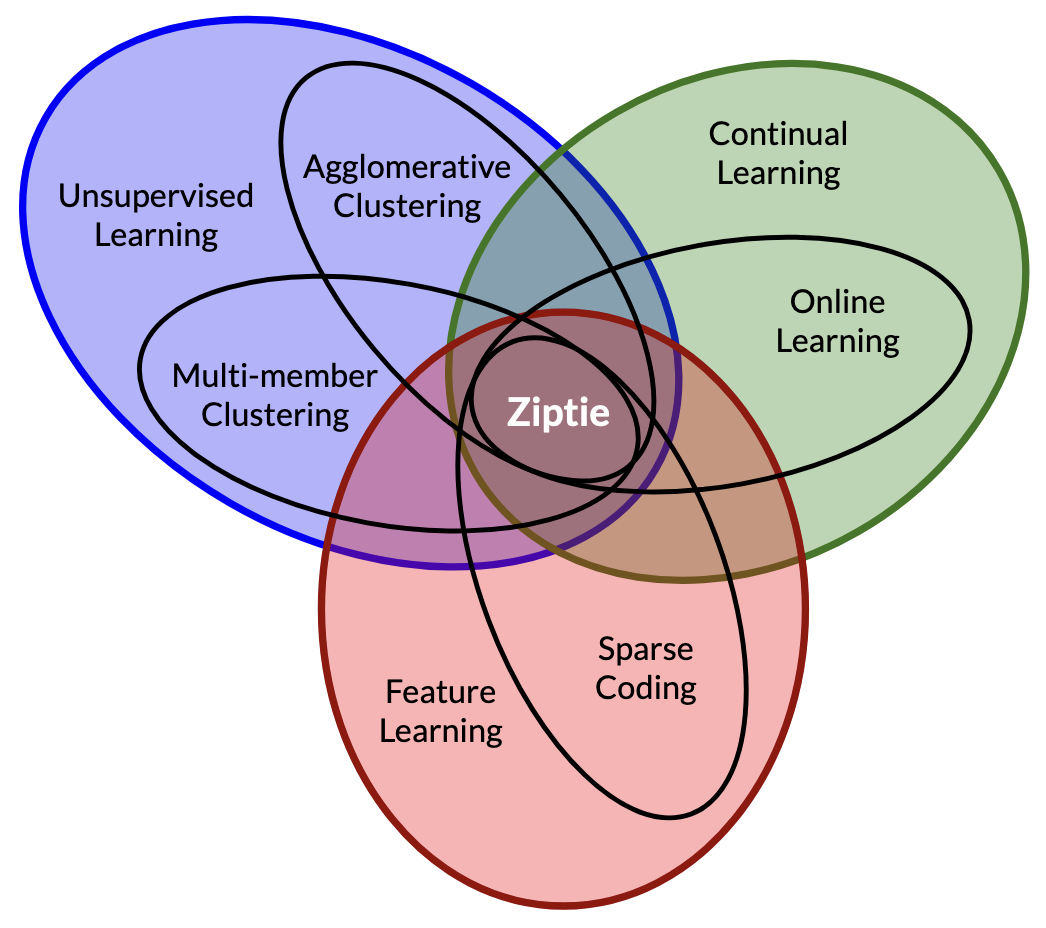
\includegraphics[width=3.0in]{images/ziptie_venn.png}}
\caption{Ziptie at the crossroads.}
\label{fig:venn}
\end{center}
\vskip -0.2in
\end{figure}

\begin{itemize}
\item{Agglomerative Clustering}
\item{Multi-member Clustering}
\item{Online Learning}
\item{Sparse Coding}
\end{itemize}
